%!TEX root = ../report.tex

\begin{document}
    \chapter{State of the Art}
	\label{chap:stateofart}
	Introduction to the modern deep learning and their impact onto the various vision tasks are described in the \nameref{sec:deeplearn} section. Information fusion in the temporal domain to fuse information is explained in \nameref{sec:tempfuse}. State of the art segmentation of the input images, in particular semantic segmentation task is illustrated in the \nameref{sec:semseg} section. State of the art segmentation in the classical era and in modern deep learning play crucial role in the temporally fused semantic segmentation. However, there is very little work of fusing the camera pose onto the segmentation task in temporal fashion. More details are discussed in the \nameref{sec:semseg}. Finally chapter \ref{chap:stateofart} is ended with the discussion on the limitations of the previous work with respect to the temporal fusion. 
	
    \section{Deep Learning}
    \label{sec:deeplearn}
    
    Deep learning is a sub field of machine learning that aims to learn the features present in the data by utilizing the hierarchical architectures. The area deep learning falls in the artificial intelligence is depicted in the picture \ref{fig:DLAI}
    
    \begin{figure}[h]
    	\centering
    	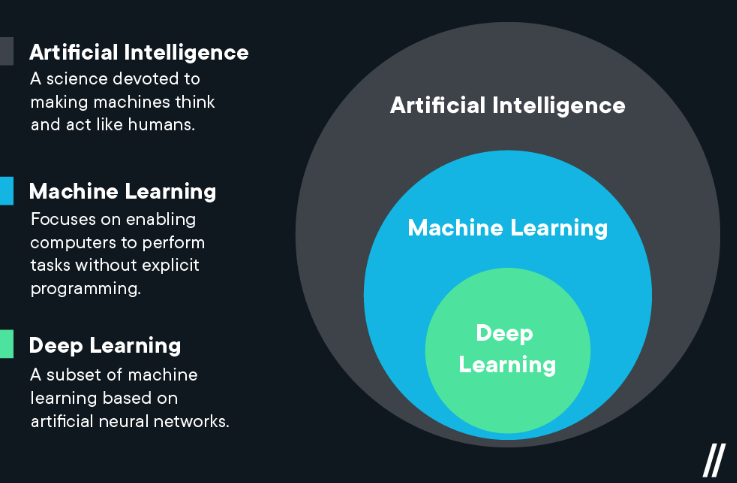
\includegraphics[width=10cm]{images/mldl.png}
    	\caption{Deep learning in the artificial intelligence domain. Courtesy of \cite{35_mldl}}
    	\label{fig:DLAI}
    \end{figure}  
    
    Classical machine learning system uses the raw input and domain expert carefully represent the data as a feature vector from which the data is fed to the models to learn the patterns and classify into appropriate classes \cite{36_lecun2015deep}. 
    Deep learning is a representation learning that takes raw data and find the patterns in the data with different levels of representation in the multiple layers \cite{36_lecun2015deep}. Deep learning can learn any complex representation of the data. For example, a image is represented as pixels and are fed to the neural network, at each layer of the network different feature are learned. In the first layer, higher level features such as edges at a specific orientation and location is determined. In the second layer motifs are learned and so on. The important aspect of the deep learning is that the features are not designed by the field expert rather than learned from the data with a specific set of learning procedures \cite{36_lecun2015deep}.
    
    Many current state of the art learning models uses the deep learning approach to learn the complex function from data. Currently deep learning method can be found in image recognition \cite{37_farabet2012learning}, speech technologies \cite{38_hinton2012deep}, discovery of drug molecule \cite{39_patel2020machine} , understanding the particle accelerator data \cite{40_ciodaro2012online}, DNA sequencing \cite{41_zhang2021deep}, ,and natural language processing \cite{42_hirschberg2015advances}. 
    
    Computer vision is the field of computer science that deals with replicating the functionalities of the human visual system. Traditionally computer vision solved the vision problem by finding the hand crafted features. However, the performance of the classical apporach is outperformed by the advancement of the deep learning based methods. Hand crafted feature descriptors such as Speeded Up Robust Features (SURF),  Hough Transforms are used as feature vectors for the classical machine learning methods for learning \cite{46_o2019deep}. Deep learning methods automatically learns the patterns from the data. Computer vision solves wide variety of problems in the perception domain. Latest approaches helps to solve the detection \cite{44_mohanty2016using}, \cite{45_han2021ecological}, classification \cite{43_srivastava2021comparative}, image synthesis and segmentation tasks \cite{47_minaee2021image}.
    
    Temporal data are the time varying information and can be commonly observed in financial portfolio management, accounting, medical records, inventory management, data from airline, hotel, train industries contains time component with it \cite{48_jensen1999temporal}. Video data are constructed from combining time variant frames and is a common example of a temporal data. Temporal fusion deals with combining of the past information into the current step computation with a aim of improved performance. 
    
    In general approach segmentation is done frame by frame or by skipping in between frames and computing the segmentation on the nth frame. Temporal fusion can be applied in these settings to perform improved segmentation task by combining the past rich information in the current step. 
     
    \section{Temporal Fusion}
    \label{sec:tempfuse}
    
	Temporal fusion can be defined as the process of fusing the temporal data onto the current step with a aim of improving the performance of the model. Temporal data can be observed in many fields such as social media, healthcare, accounting, agriculture, transportation, physics, crime data, traffic dynamics and climate science \cite{49_atluri2018spatio}. Temporal data can be encountered with different data types, Common data types are video, audio, tabular data, and sensors data. Forecasting is a common application of temporal fusion. Multi horizon forecasting is a important problem in the domain of time series. Multi horizon forecast allow the user to optimize the process across the entire path. A novel Temporal fusion Transformer (TFT) \cite{50_lim2021temporal} is a attention based DNN architecture for forecasting by fusing the important past features into the current step. Temporal fusion play a major role in the improved video action recognition. Temporal fusion helps in two ways, firstly by understanding the temporal data the accuracy of the recognition for the dynamic action is improved, secondly removing the redundant temporal data saves the computation overhead. A temporal fusion network known as the AdaFuse, fuses the current and past features with a goal of improved accuracy and efficiency \cite{51_meng2021adafuse}. A temporal non parametric fusion aims to fuse the 
	temporal pose data to the computation of the depth map thereby improving accuracy and efficiency \cite{52_hou2019multi}.  An online multi view depth prediction approach where the depth estimated in the previous step is fused onto the current step in a sensible manner. The network is named as DeepVideoMVS and it is based on the encoder decoder architecture. A ConvLSTM is placed at the latent space to fuse the information from the previous step. The proposed approach outperformed all the existing state of the art multi view stereo method evaluated on the standard metrics \cite{53_duzceker2021deepvideomvs}. 
	A Multiple Fusion Adaptation (MFA) method improves the segmentation accuracy on a unlabeled datasets. Three fusion approach was proposed under MFA, cross model fusion, temporal fusion and novel online-offline pseudo labels. The MFA produced improved semantic segmentation result of 58.2\% and 62.5\% on GTA5-to-Cityscapes and SYNTHIA-to-Cityscapes respectively \cite{54_zhang2021multiple}.  
    
    \section{Semantic Segmentation}
    \label{sec:semseg}
    
    Humans can perceive the surrounding environment and make sense of it with high accuracy. Due to the advancement of computer vision these capabilities are transferred to the machines, performing even better than humans. Today, we have computer vision models that can detect objects, find shapes, track the object movement and perform action based on the data. Computer vision is most commonly used in the autonomous driving cars, aerial mapping, surveillance applications, virtual reality and augmented reality and so on. One of the common problem in computer vision is labeling the each pixels of the image to a particular categories. Also known as the segmentation. Mathematically image segmentation can be defined as
     
    If $I$ is set of all image pixels of a image, then segmentation generate unique regions ${S_1, S_2, S_3, S_4,....S_n}$ such that combining all these regions will return $I$. 
   
    Image segmentation can be classified into three categories Semantic segmentation, Instance segmentation and Panoptic segmentation. Semantic segmentation finds the shape, size and form of the objects in addition to their location. Instance segmentation finds one more parameter of number of unique object present in the image. Panoptic segmentation is the combination of the semantic and instance segmentation. The difference between all the types of semantic segmentation can be observed in the Fig \ref{fig:SS}.
    
    \begin{figure}[h]
    	\centering
    	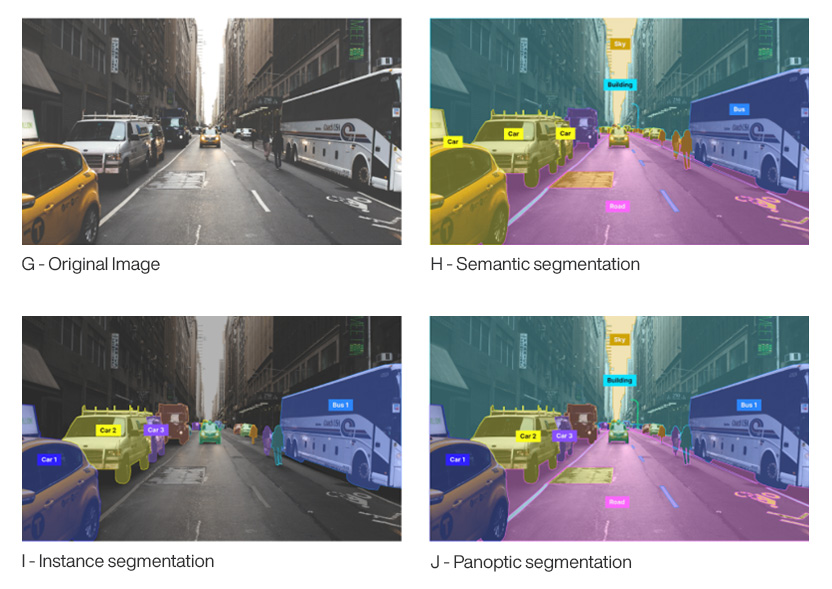
\includegraphics[width=12cm]{images/ss.jpg}
    	\caption{Semantic and Instance segmentation example. Courtesy of \cite{55_WinNT}}
    	\label{fig:SS}
    \end{figure}
    
    \subsection{Classical Semantic Segmentation}
    
    Most commonly used traditional segmentation techniques are threshold based technique \cite{56_otsu1979threshold}, histogram-based bundling, region-growing \cite{57_otsu1979threshold}, k-means clustering, watersheds, active contours, graph cuts, conditional and Markov random fields \cite{58_boykov2001fast}, sparsity based methods \cite{59_starck2005image}. However, in the recent years deep learning (DL) yielded a new generation of image segmentation models with state of the art performance. 
    
    \subsection{Deep Learning based  Semantic Segmentation}
    
    Deep learning based segmentation network can be classified into following categories \cite{60_minaee2021image}
    
    \begin{itemize}
    	\item Fully convolutional networks
    	\item Convolutional models with graphical models
    	\item Encoder-decoder based models
    	\item Multi-scale and pyramid network based models
    	\item R-CNN based models (for instance segmentation)
    	\item Dilated convolutional models and DeepLab family
    	\item Recurrent neural network based models
    	\item Attention-based models
    	\item Generative models and adversarial training
    	\item Convolutional models with active contour models
    \end{itemize}
    
    Deep learning based computer vision model most commonly use the convolutional neural network \cite{61_chen2017rethinking}, recurrent neural network (RNNs), and Long short term memory (LSTM), encoder-decoder \cite{62_badrinarayanan2017segnet} and generative adversarial networks (GANs) based networks \cite{60_minaee2021image}. The master thesis work is concentrated on the encoder-decoder based deep learning models. Encoder-Decoder based network are a two stage network that learns to map from input point to the output point. In the encoder stage the input data is compressed into a latent space representation $ z = f(x)$ and decoder decompress the latent space representation to the output $ a = g(z)$ \cite{63_goodfellow2014generative}. Latent representation of the input data in compressed form. It can be commonly observed in image-to-image translation problem as well as in sequence-to-sequence models in NLP. A reconstruction loss $ L(y, \hat{y})$ is defined at the output that measure the differences between the ground truth output $y$ and corresponding reconstruction $\hat{y}$. Autoencoders are the special version of the encoder-decoder models that have similar input and output.
    
    \begin{figure}[h]
    	\centering
    	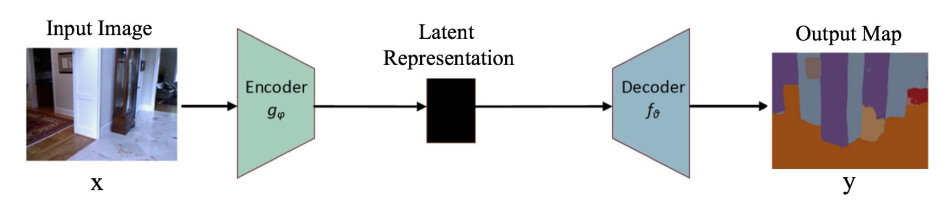
\includegraphics[width=14cm]{images/en_de.png}
    	\caption{Simple encoder-decoder architecture. Courtesy of \cite{60_minaee2021image}}
    	\label{fig:en_de}
    \end{figure} 		
    
    Most of the segmentation network are encoder-decoder based architecture. A novel semantic segmentation network was proposed by Noh et al \cite{64_noh2015learning}. The network is based on the deconvolution. The encoder network is based on the VGG 16-layer network and the decoder network takes the latent space encoding and outputs the pixel wise class probabilities. The segmentation mask and pixel-wise class labels are predicted by the deconvolutional and unpooling layers. The network generated a accuracy of 72.5 \% on the PASCAL VOC 2012 dataset. 
    
    \begin{figure}[h]
    	\centering
    	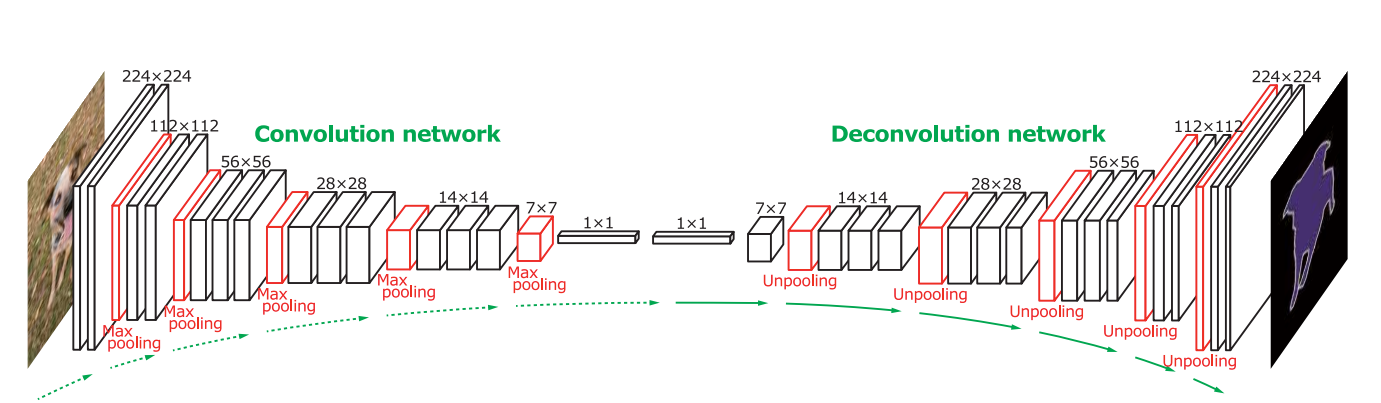
\includegraphics[width=14cm]{images/general_seg.png}
    	\caption{Simple encoder-decoder architecture. Courtesy of \cite{64_noh2015learning}}
    	\label{fig:general_seg}
    \end{figure} 
    
    Badrinarayanan et al proposed a convolutional encoder-decoder architecture for image segmentation called as SegNet. 
    
    
    \section{Temporal Fusion in Semantic Segmentation}
    Use as many sections as you need in your related work to group content into logical groups

    Don't forget to correctly cite your sources \cite{art1}.
    \section{Limitations of previous work}
    
\end{document}
